\documentclass[10pt,twocolumn]{article}

\usepackage[margin=0.72in,columnsep=0.24in]{geometry}
\usepackage{amsmath,amssymb}
\usepackage{booktabs}
\usepackage{graphicx}
\usepackage{microtype}
\usepackage{url}
\usepackage[hidelinks]{hyperref}
\usepackage{xcolor}
\usepackage{enumitem}
\usepackage{caption}
\usepackage{array}

\newcommand{\PaperAuthor}{Ivan Tyshchenko}
\newcommand{\PaperAffiliation}{Independent researcher}
\newcommand{\PaperORCID}{0009-0000-7935-6090}
\newcommand{\PaperRepository}{https://github.com/ALLPROTO/core-lm-benchmark}


\title{\textbf{VoidToken v5: Prospectively Frozen Evidence for\\
KV-Cache Compression on a Real Language Model}}
\author{\PaperAuthor\\
  \small \PaperAffiliation\\
  \small ORCID: \href{https://orcid.org/\PaperORCID}{\PaperORCID}\\
  \small \href{\PaperRepository}{\PaperRepository}}
\date{}

\newcommand{\dNLL}{\Delta\mathrm{NLL}}
\newcommand{\R}{\mathbb{R}}
\newcommand{\VTL}{\textsc{VTL5}}
\newcommand{\BF}{\textsc{BF16}}
\newcommand{\digest}[2]{%
  \texttt{\scriptsize #1}\\[-1pt]\texttt{\scriptsize #2}}

\begin{document}
\maketitle

\begin{abstract}
We report an auditable, prospectively frozen evaluation of a serialized
key-value (KV) cache codec on a pinned real language model. VoidToken v5
applies independent normalized Walsh--Hadamard transforms to the key and value
halves of each layer cache, token-wise max-absolute scaling, symmetric
quantization at 8 bits except 9 bits for layers 0 and 8, and canonical zlib
compression. The complete wire containers, including framing, metadata,
scales, and codes, are counted. The protocol fixes Qwen2.5-0.5B, WikiText-2
source windows, a canonical bfloat16 cache, wire-format byte accounting,
statistical gates, and one-shot execution rules before frozen selection and
the prospective holdout. On the registered
32-block holdout (4,096 teacher-forced predictions), complete containers
reduced canonical bfloat16 prefill-cache storage from 150,601,728 to
73,346,513 bytes ($2.05329\times$; 51.30\% fewer bytes). Relative to canonical
bfloat16-cache replay, the decoded cache produced $\dNLL=-6.09\times10^{-5}$
nat/token and 99.3896\% top-1 agreement. The one-sided 95\% block upper bound
for $\dNLL$ was 0.000549, the block lower bound for agreement was 99.2472\%,
and the Wilson lower bound was 99.1543\%; all seven prespecified gates passed.
This is a bounded artifact result for one model revision, short
teacher-forced windows, and one Apple-Silicon/MPS runtime. It is not a claim
about full-model compression, free-running generation, latency, production
serving, or state-of-the-art KV-cache quantization.
\end{abstract}

\section{Introduction}

Transformer inference stores attention keys and values so that earlier tokens
need not be recomputed. The resulting KV cache grows with layer count, sequence
length, and batch size, and is an important memory target for long-context
inference. Recent work has therefore studied low-bit quantization, outlier
handling, rotations, residual correction, pruning, and systems co-design
\cite{liu2024kivi,hooper2024kvquant,kang2024gear,jia2026saw}.

Most KV-cache papers ask how far precision can be reduced while retaining
task quality or serving speed. This paper asks a narrower question: can one
fixed codec configuration satisfy explicit quality and byte-accounting gates
under a public-freeze workflow that rejects ordinary retries within the
recorded runner and binds published outputs? The answer is positive for the
registered experiment, but the scope is intentionally small.

The contribution is primarily experimental and procedural, not a claim of a
new state of the art:
\begin{enumerate}[leftmargin=1.25em,itemsep=2pt,topsep=2pt]
  \item We specify a complete-container KV codec whose denominator, wire
        overhead, reconstruction path, and replay semantics are explicit, with
        executable checks enforcing them.
  \item We separate adaptive development from a one-shot selection phase and a
        later prospective holdout, with public Git tags and durable attempt
        markers binding code, configuration, and evidence.
  \item We publish block-level model outputs, exact artifact digests,
        recomputable confidence gates, schemas, and verifiers.
  \item We report both favorable aggregate values and the limitations that
        prevent broader model, generation, device, or serving claims.
\end{enumerate}

The final evidence tag is \path{voidtoken-v5-evidence-v1}, resolving to commit
\texttt{531e4ab8}. The full commit and scientific digests are listed in
Appendix~\ref{app:digests}. The public repository contains the source, frozen
records, and verification commands.

\section{Related Work}

\paragraph{KV-cache quantization.}
KIVI uses asymmetric quantization axes for keys and values and targets 2-bit
storage \cite{liu2024kivi}. KVQuant combines per-channel key quantization,
pre-RoPE handling, non-uniform datatypes, and sparse outlier retention
\cite{hooper2024kvquant}. GEAR combines low-bit quantization with low-rank and
sparse error correction \cite{kang2024gear}. These systems pursue compression
and inference efficiency at substantially lower nominal precision than the
8/9-bit schedule evaluated here.

\paragraph{Rotations and serving-aware designs.}
QuaRot uses randomized Hadamard rotations to suppress outliers across weights,
activations, and KV caches \cite{ashkboos2024quarot}. KVLinC applies a
Hadamard rotation plus learned linear correction for low-precision KV caches
\cite{saxena2025kvlinc}. SAW-INT4 studies block-diagonal Hadamard rotations
under paged-serving and fused-kernel constraints \cite{jia2026saw}, while
KVarN combines Hadamard rotation with variance normalization for
autoregressive reasoning traces \cite{muller2026kvarn}. VoidToken v5 also uses
a Hadamard transform, but it does not introduce rotation as a novel idea. Its
distinctive target is an artifact-level, complete-container, prospective
evaluation. Because no same-window implementations of these methods were run,
this paper makes no comparative or state-of-the-art claim.

\paragraph{Model and corpus.}
The target is the base Qwen2.5-0.5B model from the Qwen2.5 family
\cite{qwen25}. Text comes from WikiText-2, introduced with the WikiText corpus
\cite{merity2016wikitext}. Model and corpus names alone are insufficient for
reproduction, so the protocol pins repository revisions and file hashes.

\section{Registered Evaluation Target}
\label{sec:target}

\subsection{Model and corpus}

The registered suite targets \texttt{Qwen/Qwen2.5-0.5B} at pinned revision
\texttt{060db6499f32}. It has 24 layers, 14 attention heads, 2 KV heads, head
dimension 64, and hidden size 896. The runner verifies the 988,097,824-byte
weight file and its SHA-256 before loading. The full suite identifier, revision,
and digest values appear in Appendix~\ref{app:digests}.

The corpus is \texttt{Salesforce/wikitext},
\texttt{wikitext-2-raw-v1}, at pinned revision \texttt{b08601e04326}.
Rows are retained in stored order, joined with exactly two newline characters,
tokenized once without special tokens, and divided into non-overlapping
512-token blocks. There is no filtering, stripping, normalization, or index
shifting.

\subsection{Cache extraction}

For every block, tokens 0--382 form the 383-token prefill. Each layer returns
key and value tensors of shape $[1,2,383,64]$. After removing the batch axis,
the two KV heads are flattened token-major and key and value are concatenated:
\begin{equation}
  X_\ell=[K_\ell\;V_\ell]\in\R^{383\times256},
  \qquad \ell=0,\ldots,23.
\end{equation}
Native float32 cache values are rounded once through bfloat16 and restored to
float32 for computation. This canonical cache is the common input to both the
dense reference and codec. Its registered storage denominator is
\begin{equation}
  24\cdot383\cdot256\cdot2
  =4{,}706{,}304\ \text{bytes per block}.
  \label{eq:denominator}
\end{equation}
The codec therefore compresses only a batch-1, 383-token prefill KV cache. It
does not compress model weights or all process memory.

Before evaluating lossy reconstruction, two independently built canonical
cache layouts must reproduce direct-cache continuation with zero maximum logit
difference and identical top-1 decisions. This is the \emph{structural replay}
gate. It validates the extraction and reconstruction layout; it does not imply
that the lossy codec is exact.

Continuation inputs are block tokens 383--510 and targets are tokens
384--511. Each block contributes 128 teacher-forced predictions conditioned on
the supplied prefill cache.

\section{VoidToken v5 Codec}
\label{sec:codec}

For each row of $X_\ell$, the key and value halves form two independent
128-wide groups. Let $H_{128}$ be the orthonormal Walsh--Hadamard matrix. The
forward transform is
\begin{equation}
  Y_{\ell,g}=X_{\ell,g}H_{128},
  \qquad g\in\{K,V\}.
\end{equation}
No pseudo-random sign rotation is used. For every token row and K/V group, a
max-absolute quantization step is rounded to little-endian float16. Layers 0
and 8 use signed 9-bit quantization; the remaining 22 layers use signed 8-bit
quantization. Integer codes use a fixed zigzag mapping. Scale bytes and packed
codes are compressed separately with canonical zlib level 9.

Each layer is serialized as
\begin{equation}
  \texttt{"VTL5"}\;|\;\texttt{uint32-le}(m)\;|\;
  \texttt{canonical JSON}_m\;|\;\texttt{payload}.
\end{equation}
All 24 complete containers count toward the compressed-byte total, which is
the compression-ratio denominator, including magic bytes, length fields,
metadata, scale streams, and code streams. Model replay receives only arrays
reconstructed from a fresh strict parse of these serialized bytes. The parser
is a separate byte entry path, but it shares the canonical payload decoder
with the encoder self-check and is not claimed as an independent
implementation.

Figure~\ref{fig:codec} summarizes the counted wire path and the two replay
branches.

\begin{figure*}[t]
  \centering
  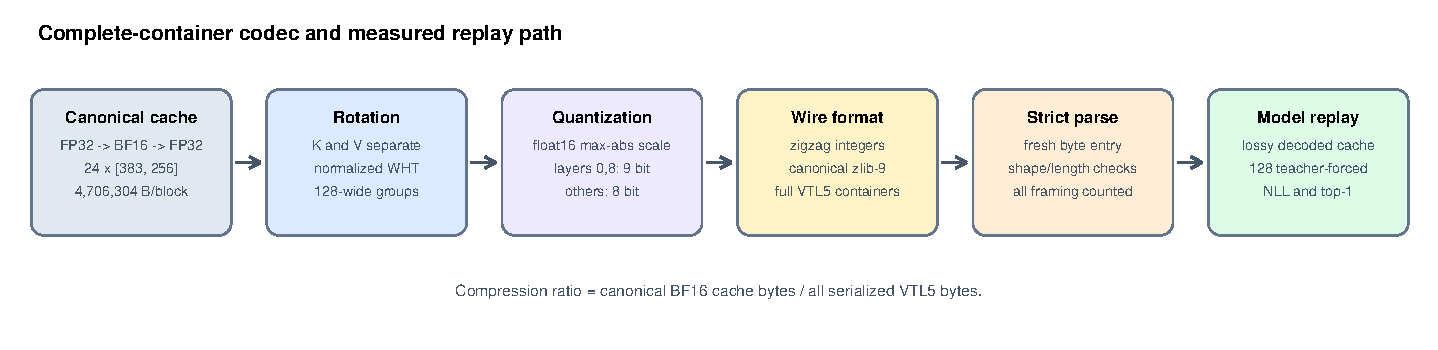
\includegraphics[width=\textwidth]{figures/codec_pipeline.pdf}
  \caption{VoidToken v5 codec and replay path. The baseline is a canonical
  bfloat16-rounded prefill cache, and the ratio counts complete serialized
  containers. The decoded model replay is lossy.}
  \label{fig:codec}
\end{figure*}

\section{Prospective Evidence Protocol}
\label{sec:protocol}

\subsection{Data partition}

The data roles are fixed and disjoint:
\begin{itemize}[leftmargin=1.2em,itemsep=1pt,topsep=2pt]
  \item validation blocks 0--31: adaptive codec development;
  \item validation blocks 32--63: one-shot frozen selection;
  \item test blocks 384--415: prospective holdout;
  \item test blocks 416--447: unscored reserve, inaccessible to the runner.
\end{itemize}
Development records are disclosed but do not count toward the prospective
verdict. The reserve is unscored, not secret or unread: corpus construction
tokenizes the complete public parquet before slicing registered windows.
Moreover, an earlier exploratory v1 pilot had already evaluated disjoint test
blocks 8--15. These facts limit the strength of any ``unseen data'' language.

\subsection{Public freezes and one-shot locks}

The fixed implementation, codec, thresholds, model, corpus, and selection
indices were published under a lightweight protocol tag at commit
\texttt{46753887}. The one-shot selection then ran at that commit. After its
PASS result and exact attempt marker were committed, a lightweight pretest tag
was published at commit \texttt{34fbd055}. Only then could the holdout runner
resolve the test split. Full tag and commit values appear in
Appendix~\ref{app:digests}.

Each frozen phase creates a fixed attempt marker with exclusive creation and
durable file and directory synchronization after environment and public-tag
checks but before resolving its registered split. An existing marker consumes
the phase. A crash after marker creation is terminal
\texttt{CONSUMED\_INCOMPLETE}; a scientific FAIL is published unchanged.
There is no ordinary retry path and no CLI option for blocks, codec parameters,
thresholds, revisions, or device.

These controls are strong process evidence, not cryptographic proof that no
person deleted a local file or ran altered private code. Git tags are also
mutable by repository administrators. The protocol therefore claims a
recorded one-shot execution corroborated by public history and artifact
binding, not an append-only trust system.

Figure~\ref{fig:timeline} shows where adaptive work ends and the frozen
selection and holdout phases begin.

\begin{figure*}[t]
  \centering
  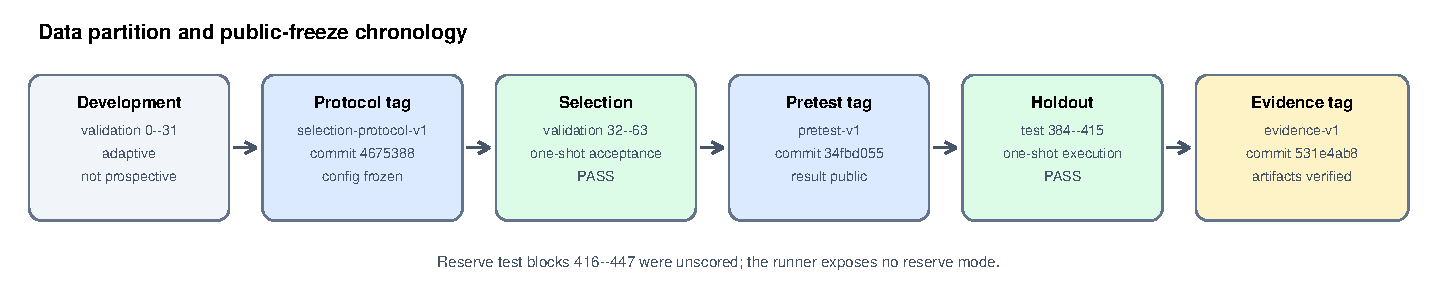
\includegraphics[width=\textwidth]{figures/protocol_timeline.pdf}
  \caption{Development, public freezes, and frozen phases. Selection accepted
  an already fixed configuration; only the later registered test blocks form
  the prospective holdout result.}
  \label{fig:timeline}
\end{figure*}

\section{Metrics and Fixed Gates}
\label{sec:gates}

For each prediction, both paths use the same target and differ only in the
prefill cache. Define
\begin{equation}
  \dNLL=\mathrm{NLL}_{\mathrm{decoded}}
        -\mathrm{NLL}_{\mathrm{canonical\ \BF}}.
\end{equation}
Top-1 agreement is agreement between decoded-cache and canonical-cache next
token decisions; it is not predictive accuracy against a benchmark label.
The complete-container compression ratio is the total denominator in
Eq.~\ref{eq:denominator} divided by the actual bytes of all 24 containers.

For $n=32$ equal-sized blocks, let $\bar d$ and $s_d$ be the sample mean and
standard deviation of block $\dNLL$. The registered one-sided upper bound is
\begin{equation}
  U_d=\bar d+t_{0.95,31}\frac{s_d}{\sqrt{32}},
  \qquad t_{0.95,31}=1.6955187825.
\end{equation}
The analogous lower bound for block top-1 rates is
$L_a=\bar a-t_{0.95,31}s_a/\sqrt{32}$. A one-sided Wilson score lower bound
over all 4,096 token decisions uses $z=1.644853627$
\cite{student1908,wilson1927}. Adjacent teacher-forced decisions are
correlated, so Wilson is a frozen workflow gate rather than independent
Bernoulli population inference. The block-level Student's $t$ bound is the
registered block-aggregated backstop, but 32 contiguous blocks still do not
define a broad population.

Selection and holdout must each satisfy all seven gates without rounding:
\begin{enumerate}[leftmargin=1.3em,itemsep=1pt,topsep=2pt]
  \item complete-container ratio $\geq2.0$;
  \item aggregate $\dNLL\leq0.01$ nat/token;
  \item $U_d\leq0.01$ nat/token;
  \item aggregate top-1 agreement $\geq0.99$;
  \item blockwise $L_a\geq0.99$;
  \item Wilson lower bound $\geq0.99$;
  \item exact structural replay on all blocks.
\end{enumerate}
Cache NRMSE, cosine similarity, maximum absolute error, and timing are recorded
diagnostics but are not acceptance gates.

\section{Results}
\label{sec:results}

\begin{table*}[t]
\centering
\caption{Registered phase results. Each phase has 32 blocks and 4,096 teacher-forced predictions. Development was adaptive and is shown only for disclosure; it does not contribute to the prospective verdict. Ratios count every serialized container byte.}
\label{tab:phase-results}
\scriptsize
\setlength{\tabcolsep}{3.1pt}
\resizebox{\textwidth}{!}{%
\begin{tabular}{llrrrrrrrrl}
\toprule
Phase & Role / blocks & Ratio & $\Delta$NLL & $\Delta$NLL U95 & Top-1 & Block L95 & Wilson L95 & Mean KL & Verdict \\
\midrule
Development & adaptive; val. 0--31 & 2.055836 & +0.0008045 & 0.0013785 & 99.5605\% & 99.3638\% & 99.3548\% & 0.0001369 & not evidence \\
Selection & one-shot; val. 32--63 & 2.054320 & +0.0005730 & 0.0012222 & 99.4141\% & 99.1762\% & 99.1827\% & 0.0001367 & PASS \\
Holdout & prospective; test 384--415 & 2.053291 & -0.0000609 & 0.0005492 & 99.3896\% & 99.2472\% & 99.1543\% & 0.0001343 & PASS \\
\bottomrule
\end{tabular}%
}
\end{table*}


Both frozen phases passed every gate. Selection compressed 150,601,728
canonical bytes to 73,309,770 bytes ($2.054320\times$), with
$\dNLL=+0.0005730$ and 4,072/4,096 top-1 agreements. Its block upper bound for
$\dNLL$ was 0.0012222; block and Wilson agreement lower bounds were 99.1762\%
and 99.1827\%, respectively.

On the prospective holdout, 150,601,728 canonical bytes became 73,346,513
complete-container bytes. This is $2.0532909\times$ compression, a reduction of
77,255,215 bytes or 51.2977\% relative to the canonical bfloat16 cache. The
baseline and decoded-cache NLL values were 2.75956684 and 2.75950591
nat/token, so $\dNLL=-0.00006093$. This small negative difference should be
read as compatibility with the fixed tolerance, not evidence that lossy
compression improves the model.

Holdout top-1 agreement was 4,071/4,096 (99.3896\%), leaving 25 disagreements.
The block upper bound for $\dNLL$ was 0.0005492, the block lower bound for
agreement was 99.2472\%, and the Wilson lower bound was 99.1543\%. The Wilson
lower bound was the closest of the three agreement gates to its threshold:
0.1543 percentage points above 99\%. Mean KL divergence was 0.00013431 nat.
Additional cache diagnostics were NRMSE 0.0032271, cosine similarity
0.99999479, and maximum absolute error 0.406687. These diagnostics do not turn
the codec into a lossless method.

Figure~\ref{fig:block-metrics} exposes the full block-level variation behind
the phase aggregates.

\begin{figure*}[t]
  \centering
  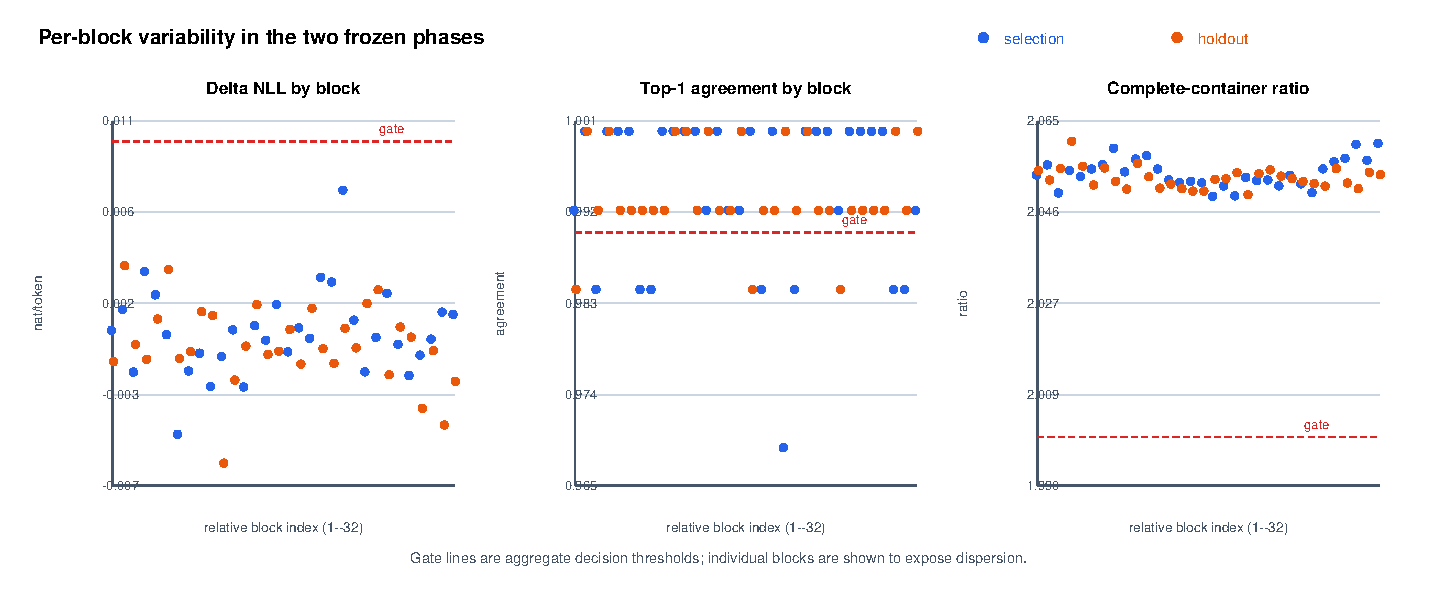
\includegraphics[width=\textwidth]{figures/block_metrics.pdf}
  \caption{All per-block records: 32 from selection and 32 from holdout. Gate
  lines show the registered aggregate decision thresholds; a block can lie on
  the unfavorable side while the prespecified aggregate and confidence gates
  still pass. No blocks were removed.}
  \label{fig:block-metrics}
\end{figure*}

The adaptive development observation was slightly stronger on top-1 agreement,
but it is not prospective evidence. Showing it in
Table~\ref{tab:phase-results} makes the tuning boundary explicit rather than
pooling all 96 blocks into a larger-looking sample.

\section{Evidence and Reproducibility}
\label{sec:provenance}

Every result contains the 32 block records, aggregate values, gate definitions,
environment versions, selected-token digest, configuration digest,
registration digest, normative implementation digest, attempt-marker links,
and a canonical result digest. The frozen implementation uses JSON Schema
validation and independently recomputes aggregate arithmetic before the
exclusive result write.

The public verifier checks schemas, canonical serialization, physical file
hashes, marker/result links, phase order, fixed source ranges, configuration
binding, per-block byte accounting, aggregate metrics, Student's $t$ and Wilson
bounds, and verdicts. In a tagged clone,
\begin{quote}\scriptsize\ttfamily
python3 \textbackslash\\
\hspace*{1em}RealLLM/verify\_voidtoken\_v5\_evidence.py \textbackslash\\
\hspace*{1em}--require-git-provenance
\end{quote}
also checks the expected commits and local tag targets. Public remote state
and chronology must be corroborated separately. This verifier validates stored
evidence; it does not rerun model inference and is not an independent external
reproduction.

The canonical holdout result starts with \texttt{d1c16e88}; the physical
\texttt{holdout.json} SHA-256 starts with \texttt{499c067d}. Both full values
appear in Appendix~\ref{app:digests}. The distinction matters because the
canonical digest excludes its own digest field, whereas the file digest covers
the exact distributed bytes.

\section{Limitations}
\label{sec:limitations}

\paragraph{Narrow experimental scope.}
Evidence covers one Qwen2.5-0.5B revision, one WikiText-2 construction, 32
holdout blocks, a 383-token prefill, 128 teacher-forced predictions per block,
and one Apple-Silicon/MPS environment. It does not establish behavior for
longer contexts, different models, datasets, prompts, batch sizes, devices, or
precision stacks.

\paragraph{Teacher forcing.}
Errors do not feed sampled token choices back into the sequence. The result
does not measure free-running or sampled generation, downstream task quality,
or long-horizon error accumulation. Top-1 agreement is reference-path
agreement, not accuracy.

\paragraph{No serving claim.}
Python encode, decode, and continuation timings are recorded but are not gates
and are not optimized-kernel benchmarks. We make no latency, throughput,
energy, peak-memory, production-serving, or economic claim.

\paragraph{No comparative baseline.}
The study does not rerun KIVI, KVQuant, GEAR, QuaRot, KVLinC, SAW-INT4, or
KVarN on identical windows. An 8/9-bit codec with approximately $2.05\times$
complete-container compression should not be read as competitive with reported
low-bit systems. The contribution is the frozen evidence procedure and bounded
artifact result.

\paragraph{Statistical dependence.}
Token decisions are correlated, blocks are contiguous corpus windows, and the
Student-$t$ calculation has only 32 block observations. Registered confidence
gates summarize this experiment; they do not prove a universal quality bound.

\paragraph{Process provenance.}
Durable markers, clean commits, source digests, and public tags constrain the
recorded workflow but cannot prove the absence of an unreported private run or
human deletion. The earlier v1 test access and full-parquet tokenization are
disclosed. External reproduction remains necessary.

\paragraph{Implementation coupling.}
The fresh strict container parser shares the canonical payload decoder with the
encoder self-check. Hash and round-trip coverage catches many faults, but a
second independent decoder would provide stronger evidence.

\section{Conclusion}

VoidToken v5 passed a prospectively frozen, one-shot holdout for complete
serialized prefill KV-cache containers on a pinned real language model. The
registered result is $2.05329\times$ compression with small NLL difference,
99.3896\% top-1 agreement, and all seven aggregate, confidence, and structural
gates satisfied. The more durable contribution is a compact evidence chain:
adaptive work is separated from prospective phases; byte accounting includes
the wire format; code and data choices are pinned; failures and incomplete
attempts are terminal; and every published number is traceable to
machine-readable records. Broader claims require multi-model, long-context,
free-running, systems-level, and independently reproduced evaluations.

\section*{Artifact Availability}

Code, frozen records, verifiers, paper source, and deterministic archive
builder are available at
\url{https://github.com/ALLPROTO/core-lm-benchmark}. The scientific evidence
state is identified by lightweight tag
\path{voidtoken-v5-evidence-v1}; the publication package is identified by
\path{voidtoken-v5-paper-v1}. Repository software is distributed under the
MIT License. The arXiv manuscript distribution license is selected separately
by the author during submission.

\bibliographystyle{plain}
\bibliography{references}

\appendix

\section{Evidence Digests}
\label{app:digests}

\begin{sloppypar}
\small
\begin{description}[
  leftmargin=0pt,
  labelindent=0pt,
  itemsep=0pt,
  parsep=0pt,
  topsep=0pt
]
  \item[] \textbf{Suite identifier:}\par
  \digest{qwen2.5-0.5b-kv-}{voidtoken-v5-prospective-v1}
  \item[] \textbf{Freeze tags:}\par
  \texttt{\scriptsize voidtoken-v5-selection-protocol-v1}\\[-1pt]
  \texttt{\scriptsize voidtoken-v5-pretest-v1}\\[-1pt]
  \texttt{\scriptsize voidtoken-v5-evidence-v1}
  \item[] \textbf{Final evidence commit:}\par
  \digest{531e4ab8d1de61ce93e83164d13caff7}{bb0759bc}
  \item[] \textbf{Protocol-freeze commit:}\par
  \digest{467538875402265b2ca915768376e2a5}{548f3069}
  \item[] \textbf{Pretest-freeze commit:}\par
  \digest{34fbd0556bd4e8fb889e628ae35175ff}{596818af}
  \item[] \textbf{Model revision:}\par
  \digest{060db6499f32faf8b98477b0a26969ef}{7d8b9987}
  \item[] \textbf{Corpus revision:}\par
  \digest{b08601e04326c79dfdd32d625aee71d}{232d685c3}
  \item[] \textbf{Configuration, canonical SHA-256:}\par
  \digest{4c7be8c836aa725722b51f66dce78af}{7a5094e887432e622b5322f7ca2cf0af8}
  \item[] \textbf{Registration, canonical SHA-256:}\par
  \digest{ad5b75791f5385740bcdd472bf81ec54}{6fa17fa59a0715a343ed91a193c1af32}
  \item[] \textbf{Normative implementation SHA-256:}\par
  \digest{55b2f589aae027e4353cf8011547d821}{a7d885d1fde8b9c3d9dd7af3cd90d783}
  \item[] \textbf{Selection result, canonical SHA-256:}\par
  \digest{11329a941051073bae9e2aec3f483f5f}{c6acf7449ed18457d020f4693c1b1876}
  \item[] \textbf{Holdout result, canonical SHA-256:}\par
  \digest{d1c16e88655c1fbc9884324742dee3f}{0b9b4bc86d973c2bf38df3a02cc090eaa}
  \item[] \textbf{Holdout result file SHA-256:}\par
  \digest{499c067d6ccff4bf1ac4a9f98436a52}{fa6c414ccced495719532347b89b46167}
  \item[] \textbf{Model weights SHA-256:}\par
  \digest{88c142557820ccad55bb59756bfcfcf8}{91de9cc6202816bd346445188a0ed342}
\end{description}
\end{sloppypar}

Both frozen phases recorded macOS 26.3 on arm64, MPS, Python 3.12.13,
PyTorch 2.13.0, Transformers 5.14.1, NumPy 2.5.1, tokenizers 0.22.2,
safetensors 0.8.0, pyarrow 23.0.1, and zlib 1.2.12. The model ran in float32;
only the reference cache was canonicalized through bfloat16.

\section{Artifact Map}
\label{app:artifact}

The machine-readable registration is
\texttt{RealLLM/v5\_registration.json}. Normative prose is
\texttt{RealLLM/V5\_PROTOCOL.md}. Adaptive records and their manifest are under
\texttt{real-llm-v5-development/}; frozen attempt and result artifacts are
under \texttt{real-llm-v5-results/}. The implementation and frozen runner are
\texttt{RealLLM/voidtoken\_v5.py} and
\texttt{RealLLM/run\_voidtoken\_v5\_frozen.py}. JSON Schemas, unit tests, an
evidence verifier with offline and Git-provenance modes, a deterministic
archive builder, and an exact SHA-256 manifest are distributed in the same
repository.

The evidence archive intentionally omits the 988 MB model weights and corpus
parquet files. Their repository revisions, byte lengths, and hashes are
registered so a reproducer can acquire and verify them separately. Exact
cross-device logits are not promised; a rerun must report its runtime and
compare scientific metrics rather than claim byte-identical MPS output.

\end{document}
